\documentclass[laboratorio]{guia}

\def \practnum {10}
\def \practica {Polarizaci\'on de la luz}

\def \materia {Laboratorio de F\'\i sica II para Qu\'\i micos}
\def \periodo {2\sptext{o} cuatrimestre de 2016}
\def \profesor {Diana Skigin}
\def \website {http://materias.df.uba.ar/f2qa2016c2}

\usepackage{graphics}
\usepackage{amsmath}
\usepackage{amsfonts}
\usepackage{graphicx}
\usepackage{float}
\usepackage{wrapfig}
\usepackage{subfigure}
\usepackage{bm}
\usepackage{grffile}
\usepackage{color}
\usepackage{framed}
\usepackage[utf8]{inputenc}
\usepackage[T1]{fontenc}
\usepackage{lmodern}
% definicion del entorno 'sabermas'
\makeatletter
\definecolor{shadecolor}{rgb}{0.89,0.91,0.94}
\newenvironment{sabermas}[1]{%
\vfill
\begin{shaded}
  \begin{center}
  {\textsection{Para saber m\'as}}
  \end{center}
  #1
\sf } 
{%
\end{shaded}%
}
\makeatother

\renewcommand{\vec}[1]{\ensuremath{\mathbf{#1}}}



\hyphenation{ coe-fi-cien-tes coe-fi-cien-te au-to-va-lor
              au-to-va-lo-res co-rres-pon-der pro-ble-ma 
              cual-quie-ra po-la-ri-za-cio-nes }

\graphicspath{{./Guia_12_Polarizacion/}}

\begin{document}
\objetivo{
    Determinar experimentalmente: (a) la intensidad lum\'\i nica transmitida
    a trav\'es de un polarizador lineal, en funci\'on de la orientaci\'on, y
    (b) el \'\i ndice de refracci\'on de un medio empleando el \'angulo de 
    Brewster.
    \tematicas{Polarizaci\'on, Ley de Malus, polarizaci\'on por reflexi\'on, \'angulo
    de Brewster.}}
\maketitle

\section{Introducci\'on}
En una onda transversal la propiedad que vibra u oscila es una magnitud de 
car\'acter vectorial y lo hace en una direcci\'on perpendicular a la 
direcci\'on de propagaci\'on. Decimos que una onda transversal est\'a 
polarizada si la propiedad que vibra lo hace de un modo predecible, es decir,
siempre paralelamente a una direcci\'on fija (polarizaci\'on lineal) o con el
vector que describe la vibraci\'on rotando a una frecuencia dada alrededor de
la direcci\'on de propagaci\'on (polarizaci\'on circular). Un ejemplo de onda
mec\'anica transversal es el caso de una onda viajando por una cuerda; aqu\'\i\
el desplazamiento o elongaci\'on es perpendicular a direcci\'on de 
propagaci\'on de la onda. La vibraci\'on puede ocurrir en cualquier direcci\'on
perpendicular a su propagaci\'on. Si se intercala una rejilla en alg\'un punto
de la cuerda, es claro que s\'olo las oscilaciones en la direcci\'on de las 
rejas podr\'an pasar. Este dispositivo, que deja pasar \'unicamente las 
vibraciones en un solo estado de polarizaci\'on se denomina {\it polarizador}.

\section{Ley de Malus}
Estudie c\'omo var\'{\i}a la intensidad de luz que recibe el detector en 
funci\'on del \'angulo entre dos polarizadores lineales empleando el 
dispositivo experimental se muestra esquem\'aticamente en la Fig. \ref{fig:1}.

La fuente de luz es una l\'ampara incandescente y el detector, un fot\'ometro.
El primer polarizador (cercano a la fuente) se denomina simplemente polarizador
y el m\'as alejado es el {\it analizador}. Este \'ultimo deber\'a tener un 
goni\'ometro para medir su posici\'on angular.

\begin{figure}[t!]
    \centering
    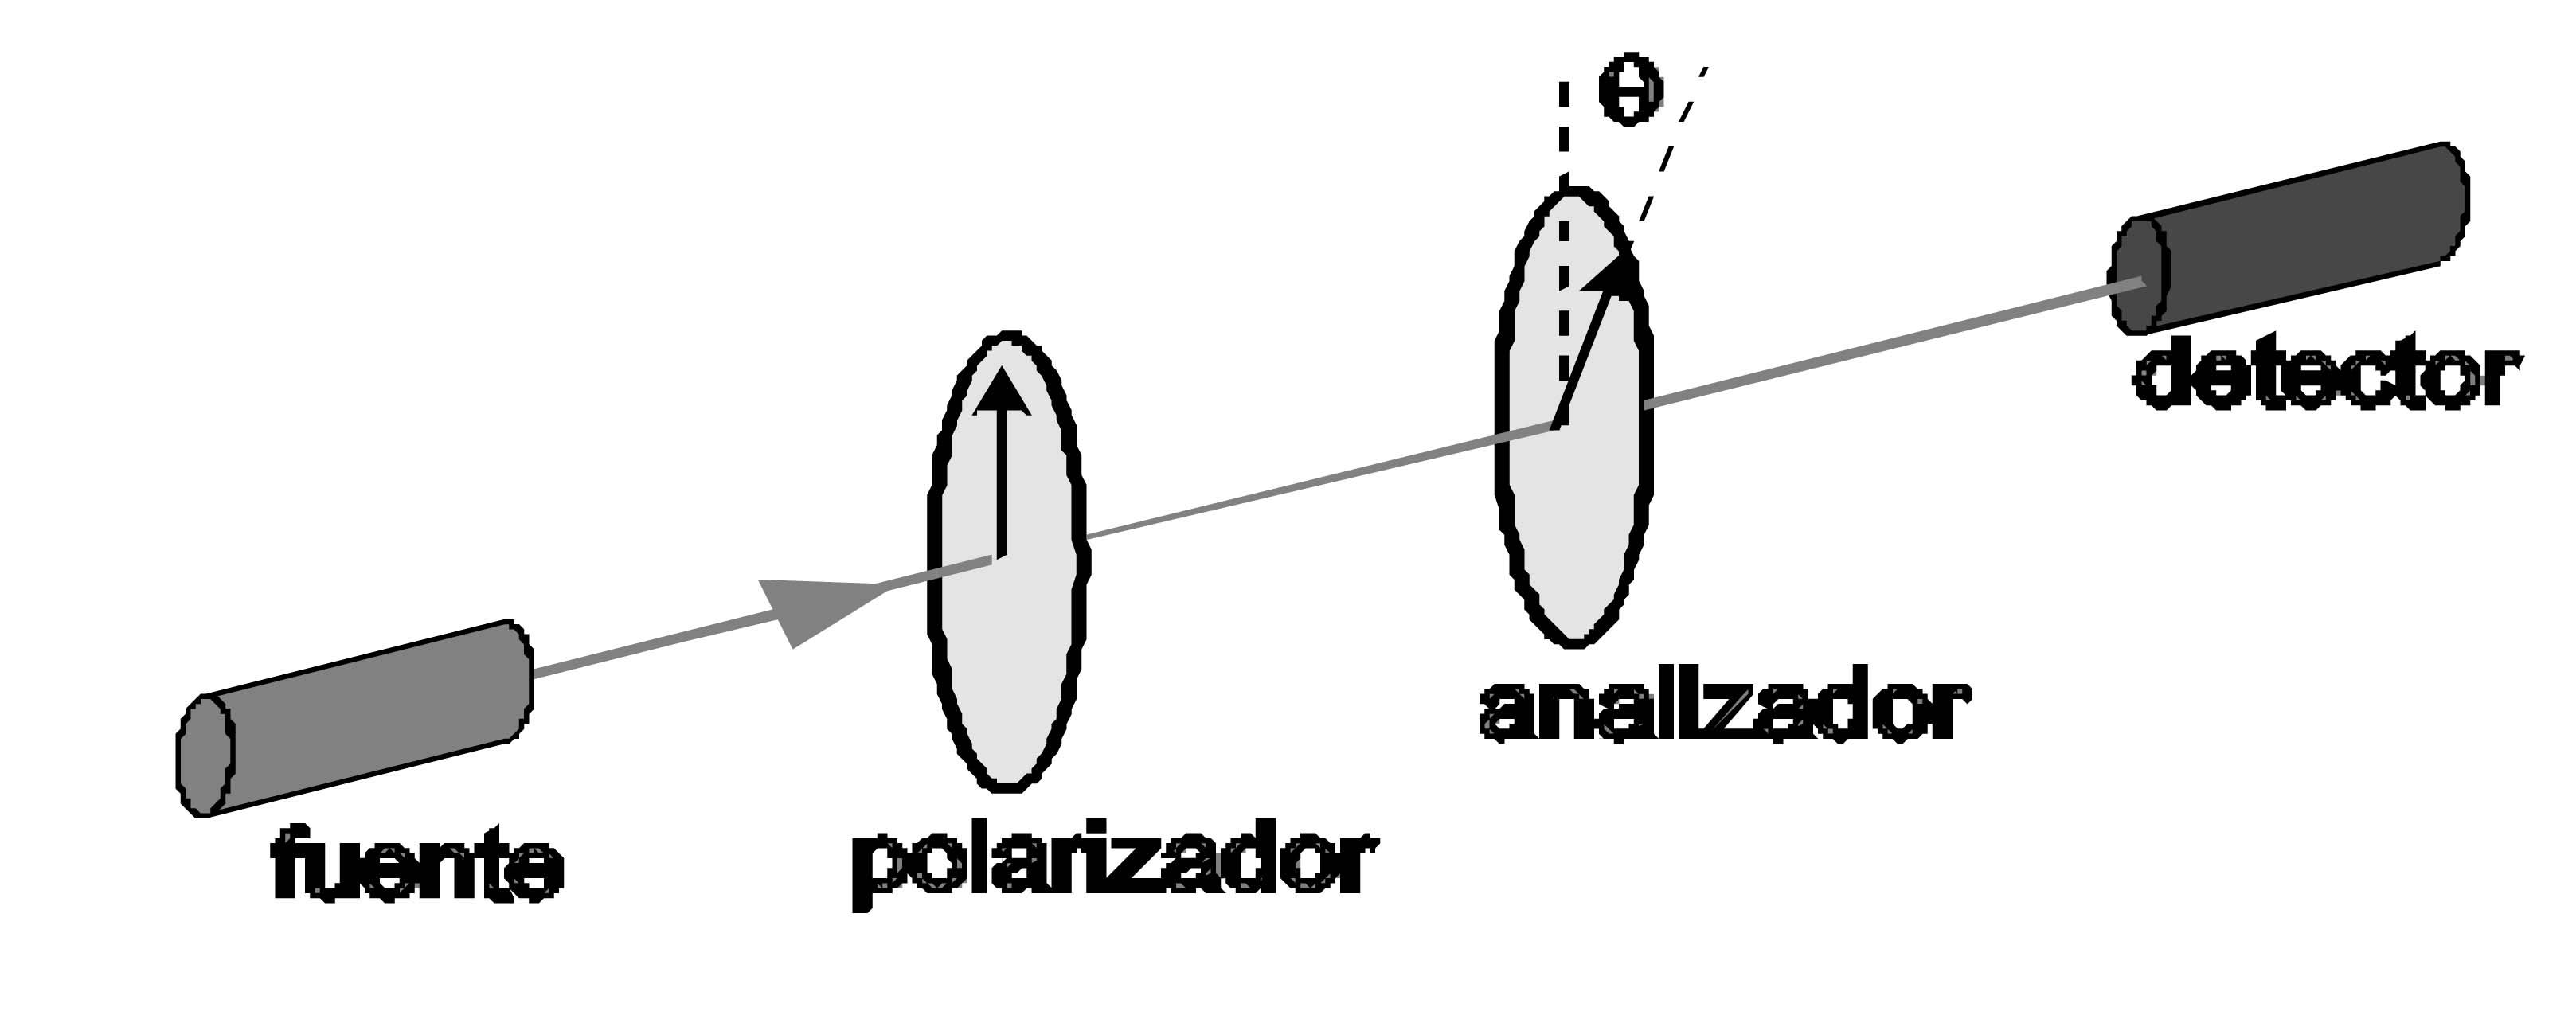
\includegraphics[width=8.5cm]{LG12--000.png}
    \caption{Esquema experimental propuesto para el estudio de la ley de Malus.}
    \label{fig:1}
\end{figure}

\section{Polarizaci\'on por reflexi\'on}

Usando l\'aser, un polar\'\i metro y el fot\'ometro, estudie las 
caracter\'\i sticas de polarizaci\'on de un haz l\'aser. ?`Es polarizada la
luz de un l\'aser de estado s\'olido? ?`Y la de un l\'aser de He-Ne? Para el
l\'aser que est\'a estudiando, si la luz es polarizada linealmente, determine
la direcci\'on de polarizaci\'on.

Usando un dispositivo similar al indicado esquem\'aticamente en la Fig. \ref{fig:2}, 
estudie c\'omo var\'\i a la intensidad de la luz reflejada y transmitida por 
una muestra de vidrio o acr\'\i lico. Para esta parte de la gu\'\i a, es 
conveniente que la muestra no sea de caras paralelas. De este modo los haces
reflejados y transmitidos por la segunda cara no llegar\'an al detector o
pantalla, proveniendo s\'olo de la reflexi\'on y transmisi\'on en una sola 
cara. Realice este estudio usando un haz l\'aser polarizado, con el campo
el\'ectrico oscilando: (a) en un plano perpendicular al plano de reflexi\'on 
(modo S) y (b) en la direcci\'on de dicho plano (modo P).

\begin{figure}[t!]
    \centering
    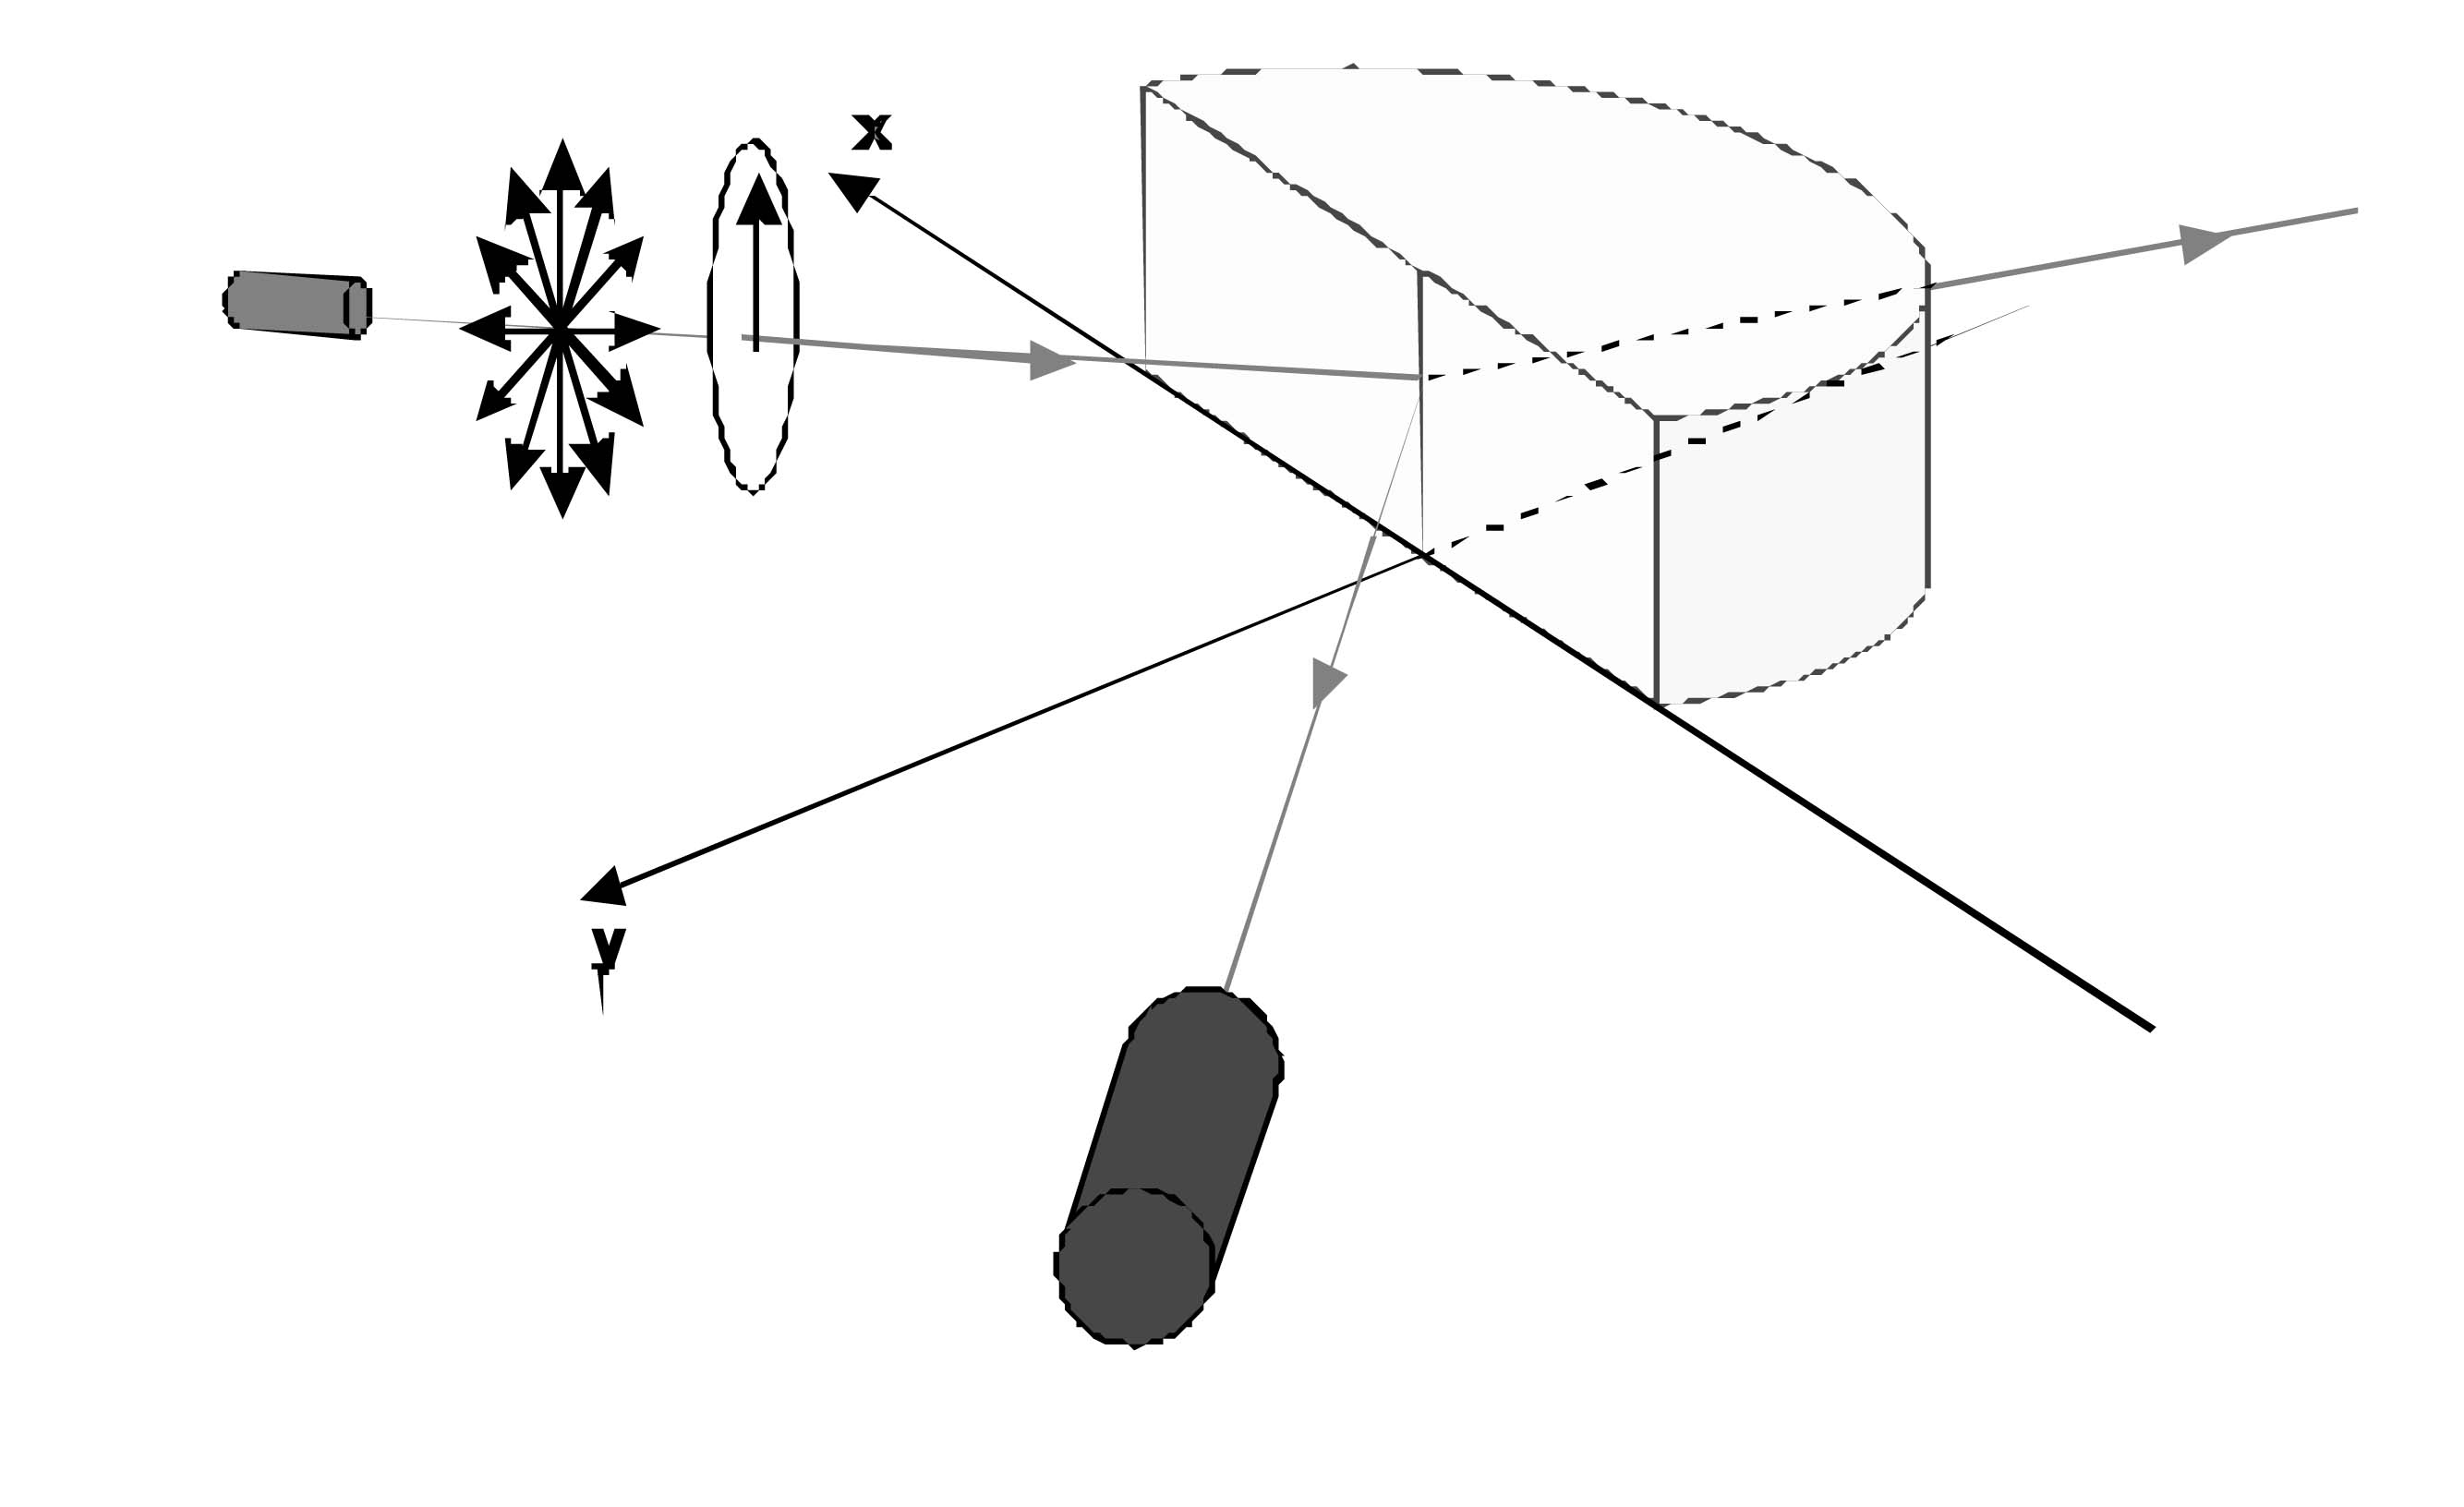
\includegraphics[width=8.5cm]{LG12--001.png}
    \caption{Esquema experimental propuesto para el estudio de la polarizaci\'on
    por reflexi\'on.}
    \label{fig:2}
\end{figure}

Empleando ahora un dispositivo similar al indicado en la misma figura, estudie
los estados de polarizaci\'on de los rayos transmitidos y reflejados, para la
situaci\'on especial en la cual el rayo reflejado y el transmitido forman 
un \'angulo de $\pi/2$~rad. Determine el \'angulo de reflexi\'on y, a 
partir de este dato, estime el \'\i ndice de refracci\'on del material. 
Discuta y explique sus resultados acerca del estado de polarizaci\'on de los
rayos reflejados y transmitidos. {\it Sugerencia: para esta parte puede 
ser conveniente usar un l\'aser con su plano de polarizaci\'on formando un
\'angulo de aproximadamente $\pi/4$~rad respecto a la perpendicular al plano
de reflexi\'on. En otras palabras, el l\'aser deber\'a tener una componente
S y otra P de magnitudes comparables. }


\nocite{Alonso1998,Hecht1986,Jenkins2001}
\bibliographystyle{unsrt} 
\bibliography{Bibliografia}

\end{document}
